\documentclass[12pt]{report}
\usepackage[letterpaper,left=3.0cm,right=3.0cm,top=2.5cm,bottom=2.5cm]{geometry}
 %\usepackage{fontspec}
 \usepackage{newtxtext}
 \usepackage{newtxmath}
\usepackage[utf8]{inputenc}
\usepackage[spanish,mexico]{babel}
\usepackage{csquotes}
\usepackage[pagestyles]{titlesec}
\usepackage{titletoc}
\usepackage{graphicx}
\usepackage{ragged2e}
\usepackage{float}
\usepackage[style=apa]{biblatex}
\usepackage{booktabs}
\usepackage[linktocpage=true]{hyperref}
% Paquetes de prueba
\usepackage{lipsum}

% Metadata
\hypersetup{pdfauthor={Nombre},
            pdftitle={Titulo},
            pdfsubject={Tesis doctoral},
            pdfkeywords={latex, doctorado, ito},
            pdflang={spanish}
            }
% Configuracion general

% Espacio entre lineas
\linespread{1.5}
% Fuente
% \setmainfont{T1}
% Espacio de parrafo
\setlength{\parskip}{8pt}
% Identacion general
\setlength{\parindent}{0pt}

% Configuracion de titulos
\titleformat{\chapter}{\centering\fontsize{16pt}{1pt}\normalfont}{\chaptername\ \thechapter}{0pt}{}%
\titleformat{\section}{\raggedright\fontsize{14pt}{1pt}\bfseries}{\chaptername\ \thechapter}{0pt}{}%
\titlespacing{\chapter}{0pt}{-20pt}{8pt}%
% Configuracion de listas de contenido
% Capitulo
\titlecontents{chapter}
  [0em]
  {}
  {\contentslabel[\thecontentslabel]{0em}}
  {}
  {\titlerule*[0.3pc]{.}\contentspage}
% Seccion
\titlecontents{section}
  [2em]
  {}
  {\contentslabel[\thecontentslabel]{0em}}
  {}
  {\titlerule*[0.3pc]{.}\contentspage}
% Figuras
  \titlecontents{figure}
  [0em]%
  {Figura~}
  {\vspace{-15pt}\thecontentslabel.\hspace{1em}}
  {}%
  {\titlerule*[.3pc]{.}\contentspage}%
% Tablas
  \titlecontents{table}
  [0em]%
  {Tabla~}
  {\vspace{-15pt}\thecontentslabel.\hspace{1em}}
  {}%
  {\titlerule*[.3pc]{.}\contentspage}%
% Traduccion de titulos
\addto\captionsspanish{
    \renewcommand{\contentsname}%
    {\fontsize{16pt}{1pt}\selectfont CONTENIDO \hfill}%
    \renewcommand{\listfigurename}%
    {\fontsize{12pt}{1pt}\selectfont LISTA DE FIGURAS \hfill}%
  \renewcommand{\listtablename}%
  {\fontsize{12pt}{1pt}\selectfont LISTA DE TABLAS \hfill}%
}
% Numero de pagina a la derecha
\newpagestyle{main}{\setfoot{}{}{\thepage}}
\pagestyle{main}
\assignpagestyle{\chapter}{main}

% Archivos de imagenes y referencias
\graphicspath{ {imagenes/} }
\addbibresource{referencias.bib}

\begin{document}

% Se incluye la portada
\begin{titlepage}
    \vspace*{-2cm}
    \begin{figure}[H]
        
\includegraphics[width=13.25cm,height=1.77cm]{portada/secretaria}
    \end{figure}

    \hrule height 3pt depth 0pt width \textwidth
    \vspace{2pt}
    \hrule height 6pt depth 0pt width \textwidth
    \vspace{2pt}
    \hrule height 3pt depth 0pt width \textwidth

    \hspace{12pt}
    \vrule height 0.7\textheight depth 0pt width 3pt
    \hspace{-1pt}
    \vrule height 0.7\textheight depth 0pt width 6pt
    \hspace{-1pt}
    \vrule height 0.7\textheight depth 0pt width 3pt

    \vspace*{-165mm}

    \begin{center}
        \textbf{DIVISIÓN DE ESTUDIOS POSGRADO E INVESTIGACIÓN}
    \end{center}

    \vspace{0.2\baselineskip}
    \begin{center}
        \fontsize{11}{12}\selectfont OPCIÓN 1.- TESIS \\
        \fontsize{12}{12}\selectfont \textbf{TRABAJO PROFESIONAL}
    \end{center}

    \vspace{0.5\baselineskip}
    \begin{center}
        \textbf{``NOMBRE DE LA TESIS''} % cambiar
    \end{center}

    \vspace{0.5\baselineskip}
    \begin{center}
        \fontsize{11}{12}\selectfont \textbf{QUE PARA OBTENER EL GRADO DE:} \\
        \fontsize{12}{12}\selectfont \textbf{DOCTOR EN CIENCIAS} \\
        \fontsize{12}{12}\selectfont \textbf{DE LA INGENIERÍA}
    \end{center}

    \vspace{0.5\baselineskip}
    \begin{center}
        \fontsize{11}{12}\selectfont \textbf{PRESENTA:} \\
        \fontsize{12}{12}\selectfont NOMBRE DEL ALUMNO % cambiar
    \end{center}

    \vspace{1\baselineskip}
    \begin{center}
        \fontsize{11}{12}\selectfont \textbf{DIRECTOR DE TESIS:} \\
        \fontsize{12}{12}\selectfont NOMBRE DEL DIRECTOR DE TESIS % cambiar
    \end{center}

    \vspace{1\baselineskip}
    \begin{center}
        \fontsize{11}{12}\selectfont \textbf{CODIRECTOR DE TESIS:} \\
        \fontsize{12}{12}\selectfont NOMBRE DEL CODIRECTOR DE TESIS % cambiar
    \end{center}

    \begin{figure}[H]
        
\includegraphics[width=2.9cm,height=3.07cm]{portada/ito_logo}
    \end{figure}

    \vspace{1\baselineskip}
    \begin{flushleft}
        \fontsize{11}{12}\selectfont \ \ \ \ \ \ \ \ \ \ \ \ \ \ \ \ \ \ \ ORIZABA, VERACRUZ, MÉXICO \ \ \ \ \ \ \ \ \ \ \ \ \ \ \ \ \ \ \ \ \ \ \ \ \ \ \ \ \ \ \ \ \ \ \ MES AÑO % cambiar fecha
    \end{flushleft}
\end{titlepage}


% Se muestra solamente hasta seccion
\setcounter{tocdepth}{1}
% Se imprimen las listas de contenido
\tableofcontents
\listoffigures
\listoftables

\chapter*{RESUMEN}
\addcontentsline{toc}{chapter}{RESUMEN}
\prechapter{RESUMEN}

\lipsum[1-2]

\makeatletter
\textbf{Palabras Clave:} \@palabras
\makeatother
% \lipsum[2-4]

\chapter*{ABSTRACT}
\addcontentsline{toc}{chapter}{ABSTRACT}
\prechapter{ABSTRACT}

\lipsum[1-2]

\makeatletter
\textbf{Keywords:} \@keywords
\makeatother

\chapter*{INTRODUCCIÓN}
\addcontentsline{toc}{chapter}{INTRODUCCIÓN}
\prechapter{INTRODUCCIÓN}

\lipsum[1-2]

\chapter*{PLANTEAMIENTO DEL PROBLEMA}
\addcontentsline{toc}{chapter}{PLANTEAMIENTO DEL PROBLEMA}
\prechapter{PLANTEAMIENTO DEL PROBLEMA}

\lipsum[1-2]

\chapter*{JUSTIFICACIÓN}
\addcontentsline{toc}{chapter}{JUSTIFICACIÓN}
\prechapter{JUSTIFICACIÓN}

\lipsum[1-2]



\chapter*{HIPÓTESIS}
\addcontentsline{toc}{chapter}{HIPÓTESIS}
\lipsum[1-2]



\chapter*{OBJETIVOS}
\addcontentsline{toc}{chapter}{OBJETIVOS}
\lipsum[1-1]

\section*{OBJETIVOS ESPECÍFICOS}
\addcontentsline{toc}{section}{OBJETIVOS ESPECÍFICOS}

\lipsum[1-1]

\chapter*{CONTRIBUCIÓN AL CONOCIMIENTO}
\addcontentsline{toc}{chapter}{CONTRIBUCIÓN AL CONOCIMIENTO}
\prechapter{INTRODUCCIÓN}

\lipsum[1-2]

\chapter*{CAPÍTULO 1: ANTECEDENTES}
\addcontentsline{toc}{chapter}{CAPÍTULO 1: ANTECEDENTES}
\chapter{ANTECEDENTES}

\lipsum[1-1] \parencite{knuth:1984}

\begin{figure}[H]
    \centering
    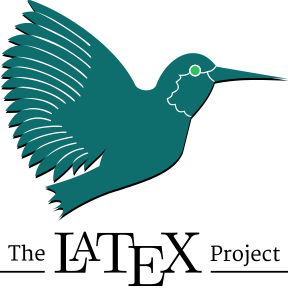
\includegraphics[width=0.5\textwidth,height=0.5\textwidth]{latex_project}
    \caption{Mi figura uno}\label{fig:fig1}
\end{figure}

\chapter*{CAPÍTULO 2: ESTADO DEL ARTE}
\addcontentsline{toc}{chapter}{CAPÍTULO 2: ESTADO DEL ARTE}
\chapter{ESTADO DEL ARTE}

\lipsum[1-3] \parencite{latex:companion}


\chapter*{CAPÍTULO 3: METODOLOGÍA}
\addcontentsline{toc}{chapter}{CAPÍTULO 3: METODOLOGÍA}
\chapter{METODOLOGÍA}

\lipsum[1-1] \parencite{latex2e}

En la \vref{tab:tabla1} podemos observar un ejemplo de tabla.

\begin{table}[H]
	\centering
	\caption{Mi tabla}\label{tab:tabla1}
	\begin{tabular}{@{}llr@{}}
		\toprule
		\multicolumn{2}{c}{Item} &                          \\ \cmidrule(r){1-2}
		Animal                   & Description & Price (\$) \\ \midrule
		Gnat                     & per gram    & 13.65      \\
		                         & each        & 0.01       \\
		Gnu                      & stuffed     & 92.50      \\
		Emu                      & stuffed     & 33.33      \\
		Armadillo                & frozen      & 8.99       \\ \bottomrule
	\end{tabular}
\end{table}

Este es un ejemplo de una referencia \cref{noexiste} y de una cita\autocite{noexiste} no encontradas.

\chapter*{CAPÍTULO 4: RESULTADOS Y DISCUSIÓN}
\addcontentsline{toc}{chapter}{CAPÍTULO 4: RESULTADOS Y DISCUSIÓN}
\chapter{RESULTADOS}

\lipsum[1-1] \cite{texbook}

\begin{figure}[H]
    \centering
    
\includegraphics[width=\textwidth,height=0.5\textwidth]{overleaf}
    \caption{Mi figura dos}\label{fig:fig2}
\end{figure}



\chapter*{CONCLUSIONES}
\addcontentsline{toc}{chapter}{CONCLUSIONES}
\prechapter{CONCLUSIONES}

\lipsum[1-2] \parencite{lesk:1977}


\chapter*{RECOMENDACIONES}
\addcontentsline{toc}{chapter}{RECOMENDACIONES}
\prechapter{RECOMENDACIONES}

\lipsum[1-2]

\chapter*{REFERENCIAS BIBLIOGRÁFICAS}
\addcontentsline{toc}{chapter}{REFERENCIAS BIBLIOGRÁFICAS}
\printbibliography[heading=none]

\chapter*{PRODUCTOS ACADÉMICOS}
\addcontentsline{toc}{chapter}{PRODUCTOS ACADÉMICOS}
\prechapter{PRODUCTOS ACADÉMICOS}

\lipsum[1-1]

\chapter*{ANEXOS}
\addcontentsline{toc}{chapter}{ANEXOS}
\lipsum[1-3]

\end{document}
